% Options here are passed to the article class.
% Most common options: 10pt, 11pt, 12pt
\documentclass[10pt]{datasheet}

% Input encoding and typographical rules for English language
\usepackage[utf8]{inputenc}
\usepackage[english]{babel}
\usepackage[english]{isodate}
% tikz is used to draw images in this example, but you can
% also use \includegraphics{}.
\usepackage{graphicx}

% These define global texts that are used in headers and titles.
\title{EC04: 16gt Item Encoder With Slime And Honey}
\author{acacia-chan}
\tags{encoders, half-speed, slime-honey}
\date{25 December 2023}
\revision{Revision 1}
\begin{document}
\maketitle

\section{Features}
\begin{itemize}
\item{Half-hopperspeed (16gt) throughput}
\item{Requires only 1 item per type per chest.}
\item{No piston toggle states.}
\end{itemize}

\section{Applications}

\begin{itemize}
\item{Encoding items}
\end{itemize}

\section{General Description}
The EC04 16gt encoder has a 16gt throughput encoder core which only requires one item per type in a chest. It uses slime and honey in its wiring. Head not included.

\vfill\break

\begin{figure}[h]
    \centering
    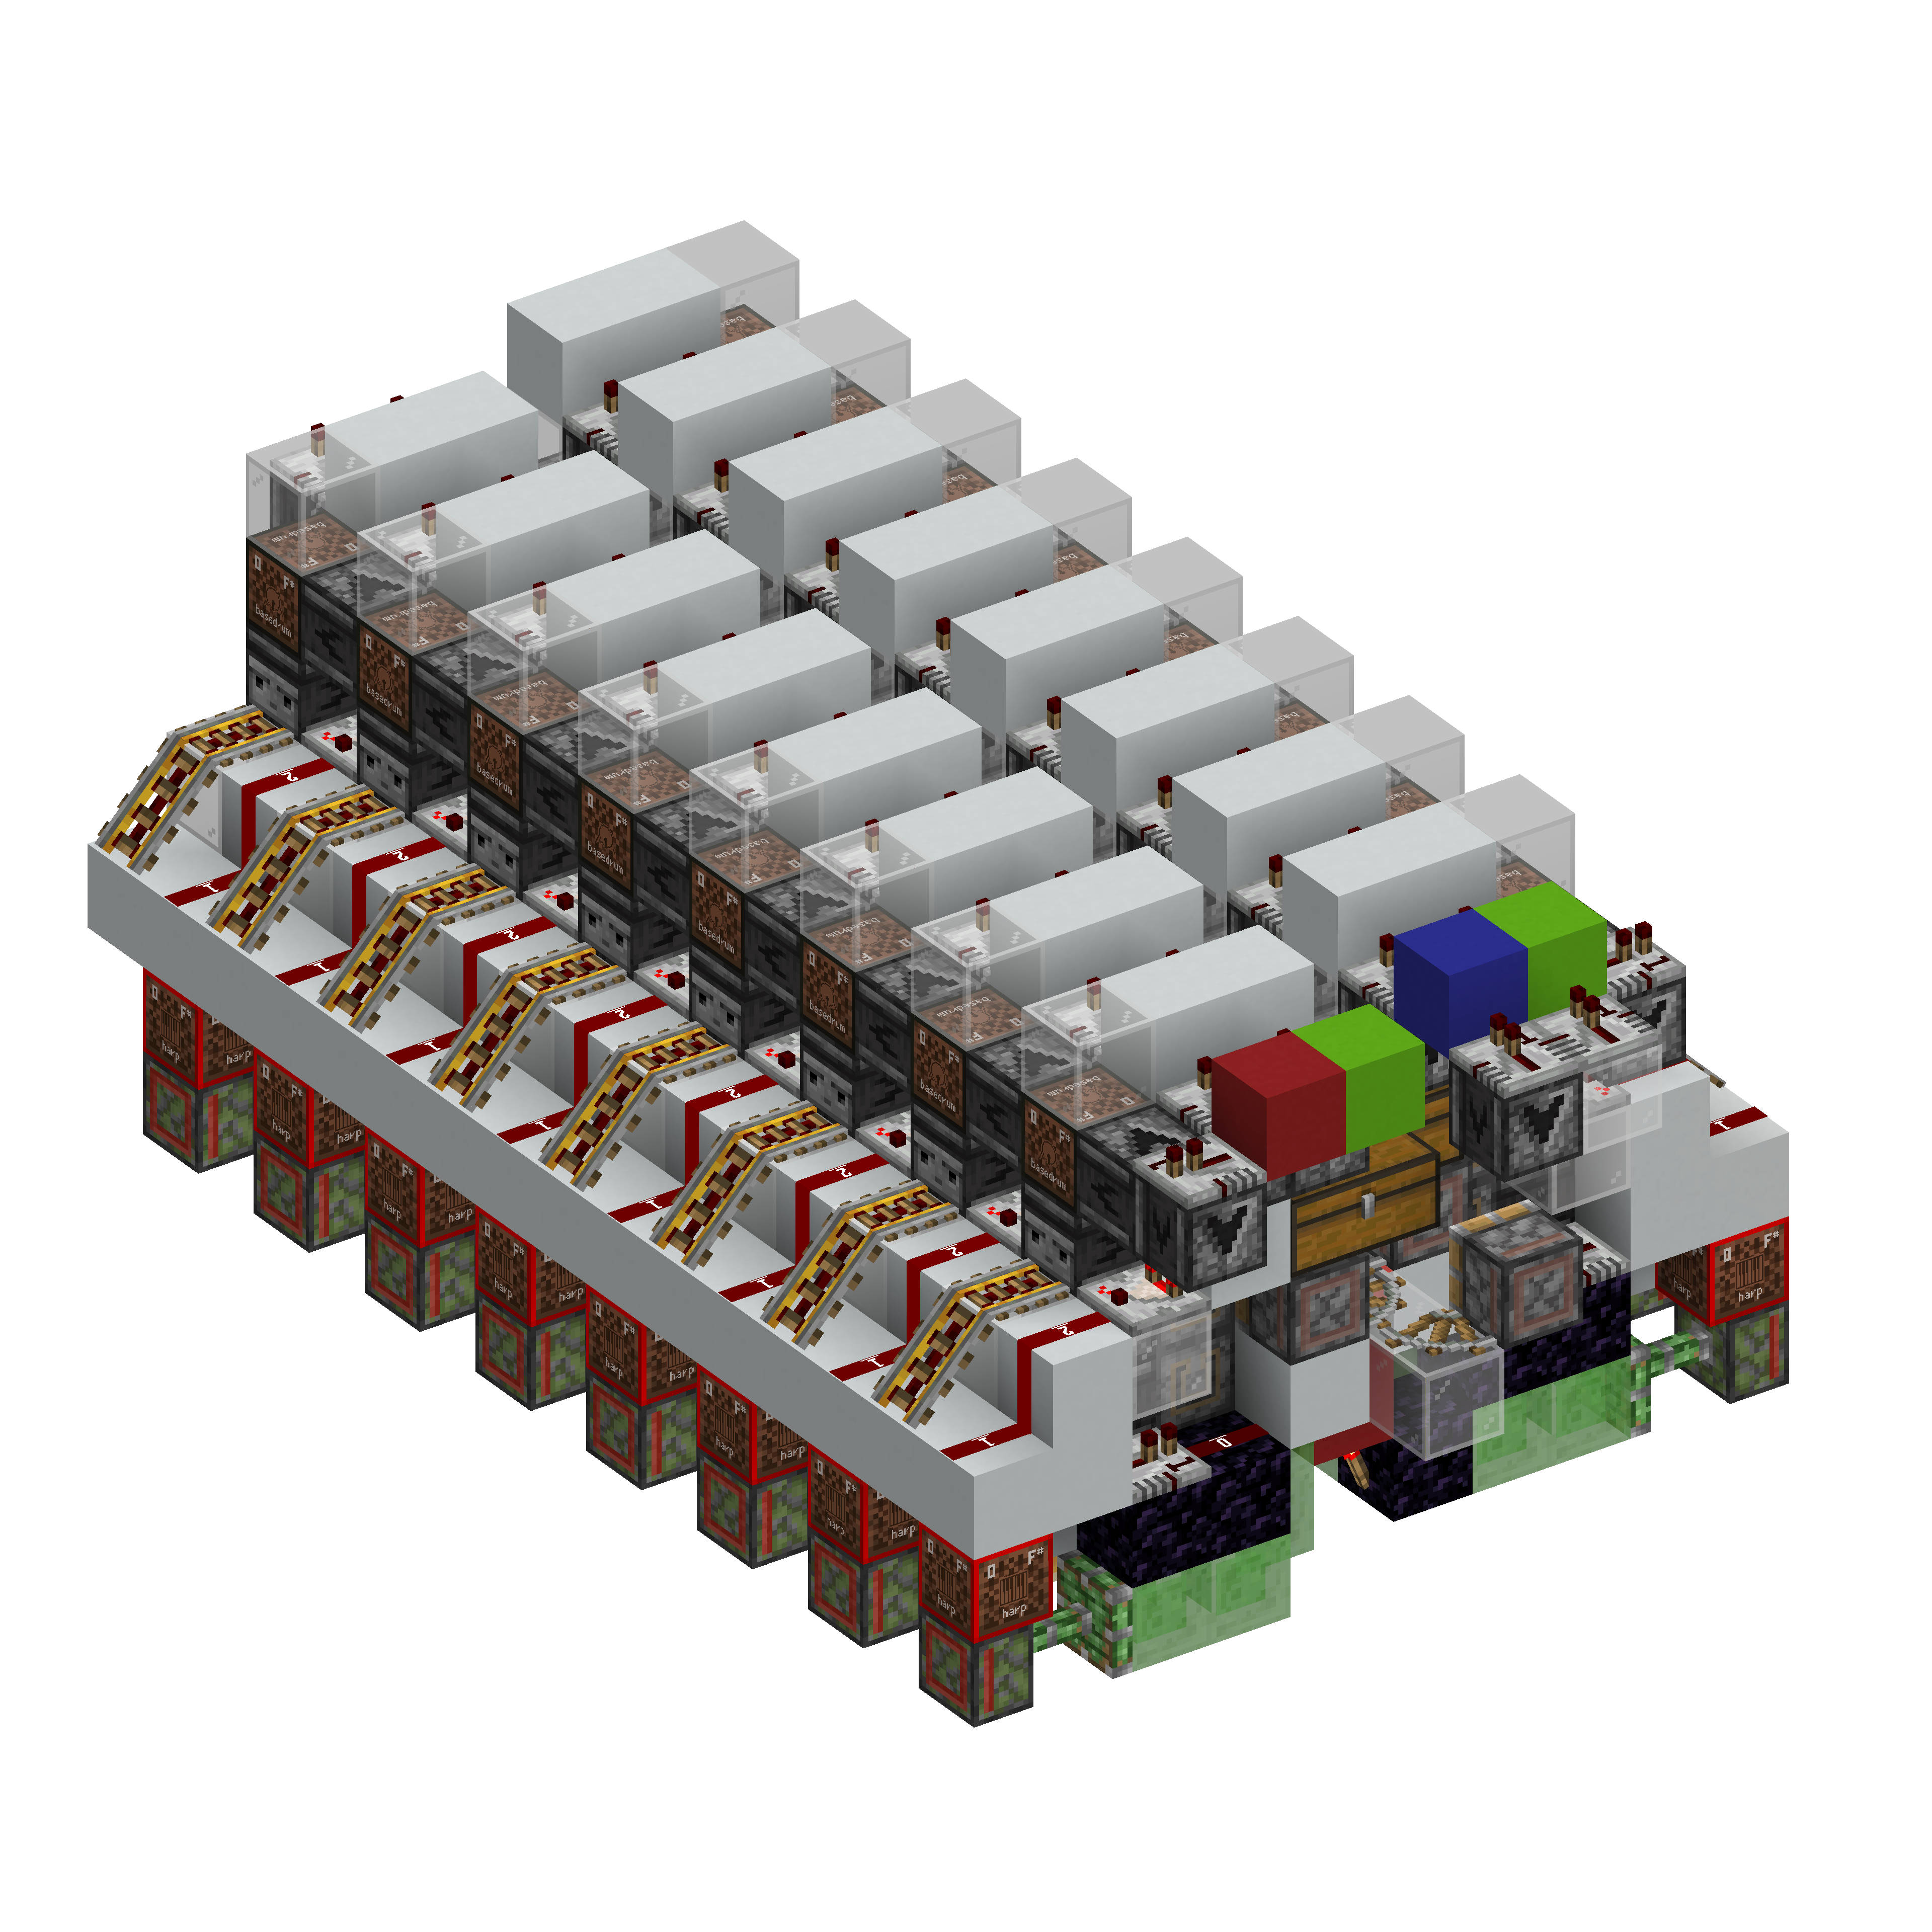
\includegraphics[width=0.48\textwidth]{area_render.png}
    \caption{\centering 16gt Item Encoder With Slime And Honey}
\end{figure}

% For wide tables, a single column layout is better. It can be switched
% page-by-page.
\onecolumn

\section{Device Specifications}

\begin{table}[h]
    \caption{Inputs}
    \begin{tabularx}{\textwidth}{l | c | X}
        \thickhline
        \textbf{Name} & \textbf{Range} & \textbf{Description} \\
        \hline
        Item input & Item & Item for encoding. \\
        \thickhline
\end{tabularx}
\end{table}

\begin{table}[h]
    \caption{Outputs}
    \begin{tabularx}{\textwidth}{l | c | X}
        \thickhline
        \textbf{Name} & \textbf{Range} & \textbf{Description} \\
        \hline
        Item output & Cart & Outputs the inputted item inside a cart. \\
        \hline
        Item Code & Code & Outputs redstone signals corresponding to mapped code. \\
        \thickhline
\end{tabularx}
\end{table}

\begin{table}[h]
    \caption{Device Specifications}
    \begin{tabularx}{\textwidth}{l | c c c | c | X}
        \thickhline
        \textbf{Parameter} & \textbf{Min.} & \textbf{Typ.} & \textbf{Max.} &
        \textbf{Unit} & \textbf{Conditions} \\
        \hline
        Throughput  & 16 & - & - & gt & Normal Usage \\
        \hline
        Active Lag & +2 & +3 & +4 & ms & At half-hopperspeed. Ryzen 5 3600, 2GB RAM. MC 1.19.3 with Lithium. \\
        \hline
        MC Version & 1.16 & 1.19.3 & - & MCV & Latest version at time of writing: 1.20.4\\
        \hline
        Dimensions & & 13 x 8 x 24 & & Blocks & \\
        \thickhline
\end{tabularx}
\end{table}
\newpage
\section{Testing Data}
\begin{table}[h]
\caption{Executed Tests}
\begin{tabularx}{\textwidth}{l | X}
    \thickhline
    \textbf{Test} & \textbf{Result} \\
    \hline
    Item encoding test & Device was able to encode with item input \\
    \hline
    Throughput test & Device was able to encode at 16gt throughput with randomized input. \\
    \thickhline
\end{tabularx}
\end{table}
\section{Download Information}
\begin{table}[h]
    \caption{Download Information}
    \begin{tabularx}{\textwidth}{l | l | l | X}
        \thickhline
        \textbf{Identifier} & \textbf{MC} & \textbf{File} & \textbf{Description} \\
        \hline
        EC04 & 1.19.3 & \href{https://github.com/Soontech-Annals/Archive/blob/8413f90a054b6c415703bae02badeba7541344f6/Archive/encoders/EC04\%2016gt\%20Item\%20Encoder\%20With\%20Slime\%20And\%20Honey/EC04\_16gt\_Item\_Encoder\_With\_Slime\_And\_Honey.litematic?raw=1}{EC04\_16gt\_Item\_Encoder\_With\_Slime\_And\_Honey.litematic} & Schematic of device. \\
        \hline
        \thickhline
    \end{tabularx}
\end{table}

\end{document}

